\section{Enhedstest software}
Til test af softwaren til systemet er enhedstests benyttet. Enhedstest er den test metode hvor softwaren deles op i mindst mulige dele og tests helt isolerede fra resten af systemet. Under enhedstest sikres at hver enhed i systemet fungere efter hensigten. Enhedstest bliver udarbejdet samtidig med produktions koden  bliver udviklet, på den måde bliver de fleste fejl i systemet fanget, mens systemet er under udvikling. Dvs fejl i systemet bliver opdaget samtidig med at systemet er under udvikling, hvilket mindsker fejlens omfang og omkostninger for at rette fejlen.

På figur \ref{fig:test_forlob} ses mængende af fejl i div testforløb og fokus opdelningen.
\begin{figure}[H]
	\centering
	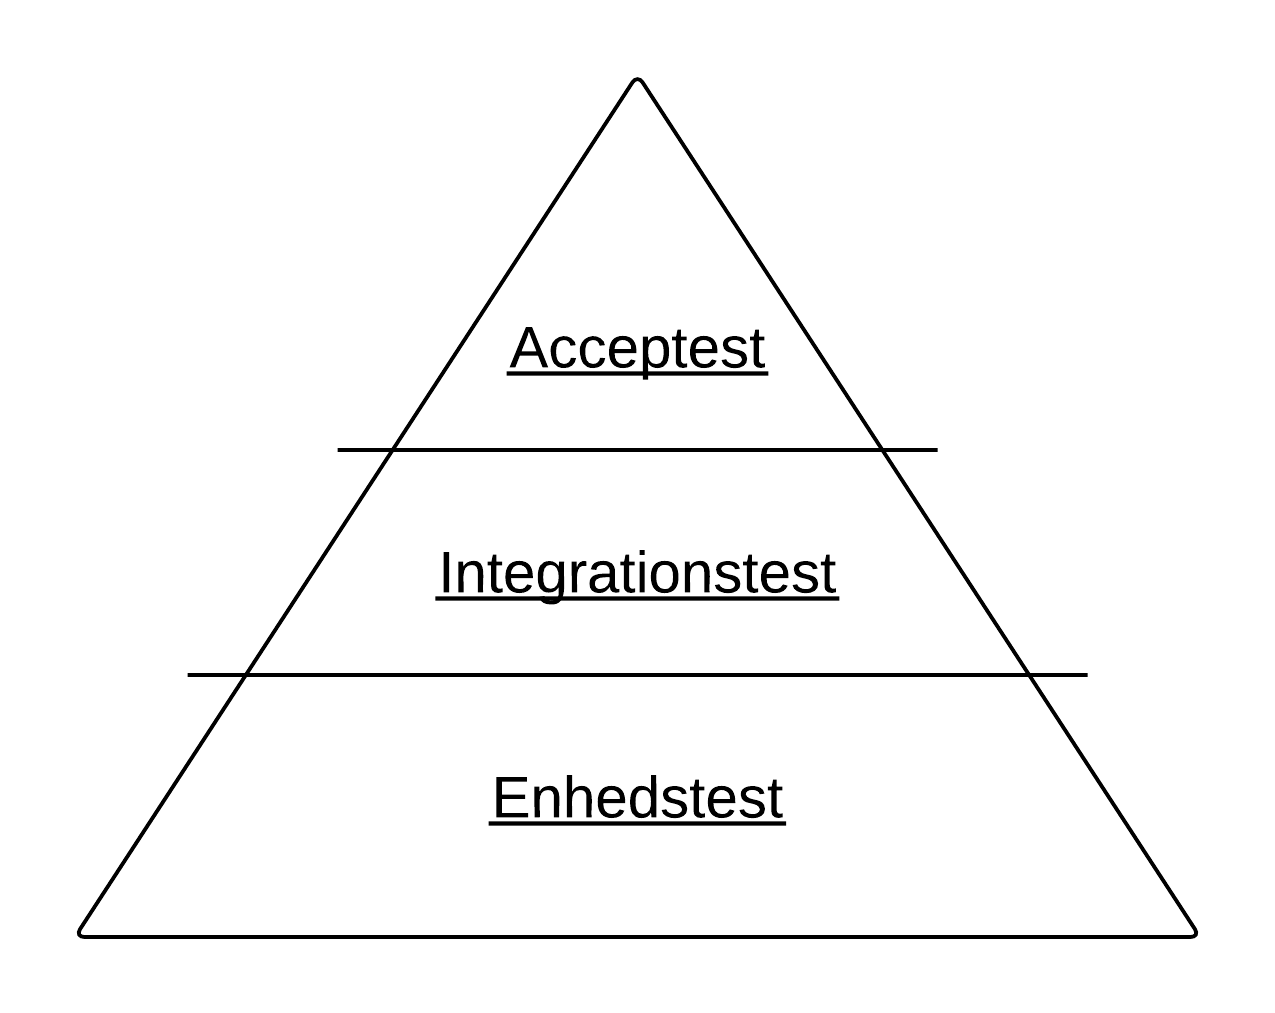
\includegraphics[width=0.6\textwidth]{Billeder/Test/forlob.png}
	\caption{Mængden af fejl}
	\label{fig:test_forlob}
\end{figure}

\subsection{Test opbygning}
Enhedstestene er opbygget efter AAA-modellen\footnote{http://c2.com/cgi/wiki?ArrangeActAssert}.\\ 
Arrange: \\
Her opsættes input til testen, eller evt afhængigheder håndteres. \\
Act: \\
Her bliver det ønskede kode stimuleret. \\
Assert: \\
Her forventes et bestemt output og testen afgøres om den er succesfuld eller ej.

\newpage
På  figur \ref{fig:aaa} ses et eksempel på AAA modellen. I testen bliver der testet for om den korrekte metode bliver kaldt når bruger prøver at logge in på webapplikationen. 

\begin{figure}[H]
	\centering
	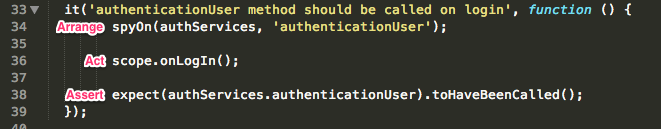
\includegraphics[width=0.6\textwidth]{Billeder/Test/aaa.png}
	\caption{AAA eksempel}
	\label{fig:aaa}
\end{figure}